\section{Bmboot architecture}

Figure~\ref{fig:components} illustrates a typical application, consisting of a Linux counterpart and a bare-metal counterpart. The core or cores running Linux (collectively the \textit{Linux Realm}) take the role of managing the \textit{executors} -- cores dedicated to executing bare-metal programs.

Bmboot provides a number of key components enabling this workflow, described in the following sections.

\begin{figure}[h]
  \centering
  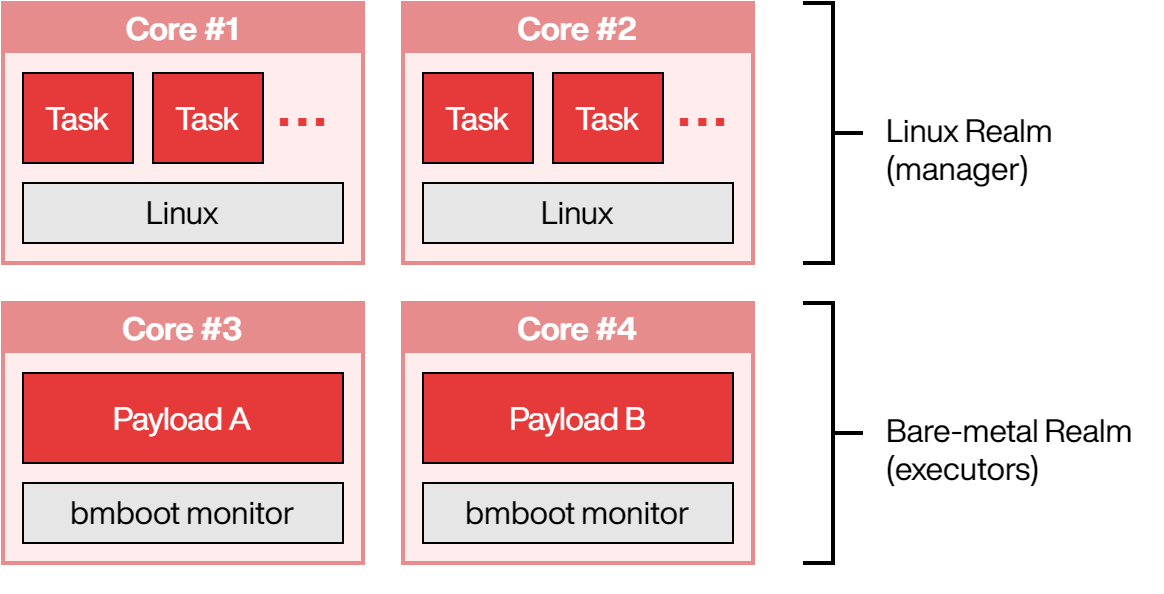
\includegraphics[width=0.8\textwidth]{images/realms-simplified.png}
  \caption{Components in a complete system using Bmboot \label{fig:components}}
\end{figure}

\subsection{Core components}

\subsubsection{Payload}

Payload is the user's real-time application. It executes under the supervision of the monitor and can make use of APIs provided by the monitor. To function properly, the payload must respect the execution environment and must be compiled in a prescribed way.

\subsubsection{Bare-metal monitor}

The bare-metal monitor executes on the same core as the payload. It starts the payload and provides services to it via an API. The monitor can be called upon to interrupt the execution of the payload, but otherwise does not interfere with it during normal execution.

\subsubsection{Payload runtime library}

The monitor's API is exposed to the payload through a small library of functions that is linked into the payload. Internally, it makes use of a mechanism similar to the \textit{syscall} in a traditional OS to change the execution context from user application into the monitor.

\subsubsection{Manager library and command-line tools}

On the Linux side, an application can control the life-cycle of the bare-metal application through a library that is provided. Alternatively, if the bare-metal application is able to function without a Linux counterpart, it can be managed using a provided command-line tool (\texttt{bmctl}).

\subsection{Memory organization and management}

\begin{figure}[h]
  \centering
  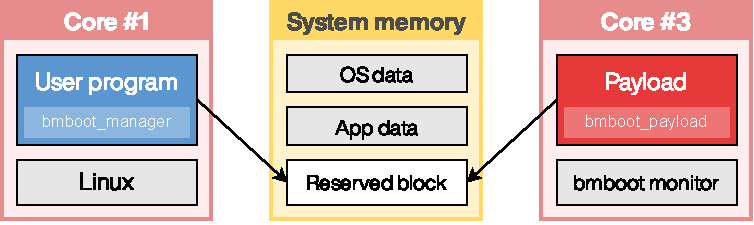
\includegraphics[width=0.9\textwidth]{images/memory-arch.pdf}
  \caption{Each executor has a dedicated block of memory for communication with the manager}
\end{figure}

The design is based on the assumption of a cache-coherent memory system. Regions of physical memory are marked as ``reserved'' in the system device tree; this excludes them from being managed by Linux and makes them safe to use by bare-metal code.

The need for manual address allocation and modification of the device tree in an inconvenience, but there is a number of reasons for it:

\begin{itemize}
    \item Monitor and payload binaries are non-relocatable -- the run-time layout of the physical memory must already be known at the time when these binaries are built.
    \item The alternative to modifying the device tree would be to have a kernel driver allocate some contiguous physical memory. Maintaining a kernel driver is not a trivial task and we prefer to avoid it.
    \item A predictable memory layout reduces the number of ``moving parts'' and simplifies debugging.
\end{itemize}

Each Bmboot-controlled CPU core requires its own instances of the following memory regions:

\begin{itemize}
    \item monitor binary (all-inclusive: code, static variables, stack, heap)
    \item an \textit{IPC Block} between the monitor and manager
    \item payload binary
\end{itemize}

It is expected that a typical user application will additionally dedicate some memory to exchange application-specific data.

Note: No memory protection is implemented at the time of writing.

\subsubsection*{FGC4 specifics}

\begin{enumerate}
    \item To ease the task of memory assignment, FGC4 includes a utility called \texttt{mmtool} to generate C/C++ headers and linker scripts with addresses of the various memory regions.
    \item A relatively large chunk of physical memory is dedicated to a so-called \textit{pool}. When the application starts, blocks are allocated from the pool for various purposes like log buffers.
\end{enumerate}

% To review: https://github.com/ceph/dpdk/blob/master/lib/librte_eal/linuxapp/eal/eal_memory.c

\subsubsection{Cache concerns during application startup}

A fundamental assumption in the design of Bmboot is that the memory system is cache-coherent. That is, when one CPU core writes to a physical memory location, other cores subsequently reading from the same location will observe the new value. Moreover, the observed order of memory operations is the same for all cores.

The CPU provides hardware support for cache coherence, by means of the \textit{Snoop Control Unit} (SCU). However, there are prerequisites that must be satisfied: the memory must be configured as cacheable by all participants, since uncached accesses are not broadcast to other cores.
The insidious thing is that with incorrect setup, the programs might still execute correctly due to luck -- until a small change is made and suddenly they don't.

When the Bmboot monitor is started for the first time, the core is in its default reset configuration, which disables all caches. One of the first steps is to enable caching, so that future memory operations are coherent. Until that point has been reached, care must be taken to manually flush each range of memory modified by one core and read by another.

\subsection{Executor state machine \label{subsec:executor-fsm}}

When a CPU core is put under the control of Bmboot, it becomes an \textit{executor domain}\footnote{The terminology was inspired by the Xen hypervisor, where a \textit{domain} refers to a virtual machine. In Xen, domains can be created at will, while in Bmboot, there is a fixed number of domains corresponding one-to-one to the available CPU cores.}, or simply \textit{executor}. The lifecycle of an executor is controlled by the monitor, based on commands from the manager, following the state machine depicted in Figure~\ref{fig:state-machine}.

\begin{figure}[h]
  \centering
  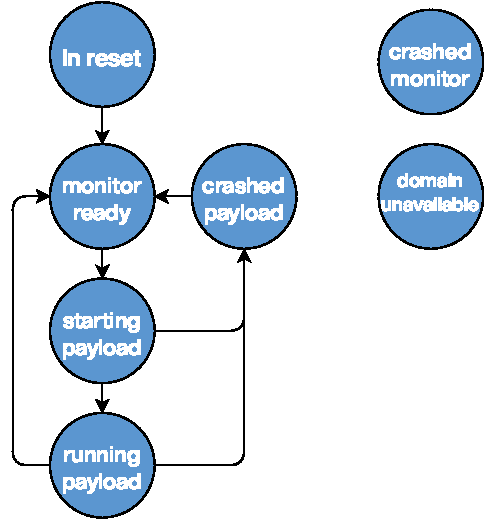
\includegraphics[width=0.55\textwidth]{images/executor-fsm.pdf}
  \caption{Executor domain state machine \label{fig:state-machine}}
\end{figure}

At the beginning, an executor core must be in power-on reset. Otherwise, the manager will determine that there is already other code executing (perhaps the core is being used by Linux) and will deem the domain \textit{unavailable}.

It is important to note that no persistent state is being kept on the manager side; every time a new access to a domain is initiated (whether through the \texttt{bmctl} utility or the \texttt{IDomain::open} API function), it is necessary to determine whether the domain is under the control of Bmboot or not. This process is described by Figure~\ref{fig:state-determination}: if the CPU core in question is already executing code, a specific signature value, placed at a fixed memory address, is used to distinguish between a core under Bmboot control and a core executing other code. This is a heuristic approach; a challenge--response mechanism would provide more confidence. However, this would conflict with the design requirement to not interrupt a running payload unless it needs to be terminated.

\begin{figure}[h]
  \centering
  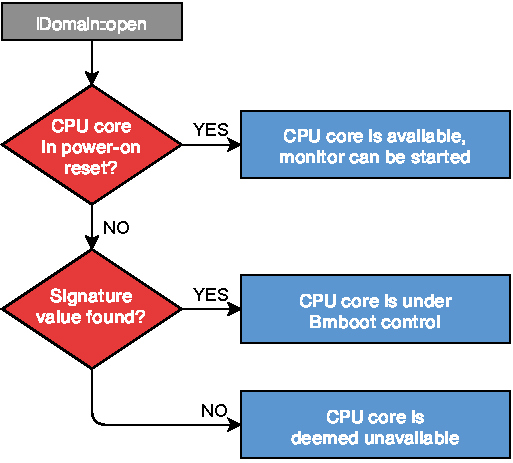
\includegraphics[width=0.65\textwidth]{images/state-determination.pdf}
  \caption{Executor domain state determination flow chart \label{fig:state-determination}}
\end{figure}

\subsection{Communication between manager and monitor}

The manager issues commands to the monitor through the IPC block. Commands are only processed when the domain is in \texttt{monitor ready} state. Only one command is currently implemented, \texttt{start payload}.

A different approach is necessary when the manager needs to terminate a running payload, since the monitor is not active in this state, and commands are therefore not being executed. For this purpose, an intrusive mechanism called \textit{inter-processor interrupt} (IPI), described further in subsection~\ref{ssec:ipi}, is used.

\subsection{Payload execution environment}

Bmboot payloads execute in an environment with many similarities to other embedded platforms without operating system.

It is possible to use many functions from the C standard library, and even some functions from POSIX including:

\begin{itemize}
    \item math functions
    \item string functions
    \item memory allocation
    % \item \texttt{usleep}
    \item standard output (\texttt{printf} et al.)
\end{itemize}

Many classes from the C++ Standard Template Library are also safe to use:

\begin{itemize}
    \item containers (array, map, vector)
    \item strings
    \item utility classes, such \texttt{std::optional}
    \item exceptions
\end{itemize}

On the other hand, the following facilities are \textit{not} available:

\begin{itemize}
    \item file I/O
    \item standard input
    \item threads
    \item signals
    \item networking
\end{itemize}

The technical explanation is that only those parts of the library that do not depend on \textit{syscalls} can be safely used. As there is no operating system, the majority of syscalls are not available, and this extends to any functionality relying on them. Some syscalls are available, either by emulating them inside the payload runtime (\texttt{\_sbrk}) or by calling into the monitor (\texttt{\_write}).

Caution must be exercised when using dynamic memory allocation, especially indirectly (e.g., \texttt{std::vector}). As there is no virtual memory, the environment is particularly prone to memory fragmentation, which over time limits the maximum size of a contiguous block that can be allocated, regardless of the total free memory.

Payloads execute in a flat memory space. The particular load address will depend on which CPU is executing the payload. By default, the program will be able to access all of physical memory. This includes parts of the address space which do not correspond to valid memory and which can destabilize the system if an access is attempted.
